\documentclass[10pt, letterpaper]{article}
\usepackage[top=80pt,bottom=80pt,left=60pt,right=60pt]{geometry}
\usepackage{tabularx}
\usepackage{float}
\usepackage{amsmath} % for boxing equations
\usepackage{titling}
\newcommand{\subtitle}[1]{
  \posttitle{
    \par\end{center}
    \begin{center}\large#1\end{center}
    \vskip0.5em}
}
\usepackage{tikz}
\usepackage[section]{placeins}
\usepackage[utf8]{inputenc}
\usepackage{pgfplots} % for table
\usepackage{pgfplotstable} % for linear regression
\usepackage{csvsimple}
\usepackage{subfig}
\usepackage{setspace} % line spacing
\doublespacing

\begin{document}

  \title{Internal Assessment: The Monte Carlo Method}
  \subtitle {IB Math HL Period 5, Dr. Silverman}
  \date{16 November 2015}
  \author{Jackson Chen}
  \maketitle

  \section{Introduction}

  \subsection{Personal Engagement}

  I have always learned to solve numeric problems, such as calculating the area of a shape in Euclidean geometry,
  with an exact, formulaic method. This may consist of using numeric relationships or calculus. However, I became fascinated with
  the Monte Carlo method after learning about it from a professor. I had never thought of applying probability to numeric problems
  with seemingly definite solutions until then. The Monte Carlo method will be described in more detail in Section \ref{subsec:explanation}.
  This method is also surprisingly straightforward compared to some of
  the other methods used to solve numeric problems, and may have even an advantage when finding areas of irregular shapes.

  \subsection{Explanation} \label{subsec:explanation}

  The Monte Carlo method consists of using random sampling in order to solve numerical problems. This may seem like an imprecise method
  of solving, for example, the area of a circle. However, there are two crucial criteria to consider when using the Monte Carlo method:
  \begin{itemize}
    \item The greater the number of random inputs that are chosen, the greater the accuracy
    \item The more uniform the distribution of random samples, the more accurate the final answer
  \end{itemize}

  In order to address the second point made in the list above, one may assume that truly random numbers are needed to ensure a fair distribution.
  However, this is not the case as pseudorandom number generation, which is prevalent in many number generator algorithms, should be satisfactory
  for many instances of the Monte Carlo method.

  \section{Sample Calculation} \label{sec:usage}

  A sample calculation for the Monte Carlo Method will be performed to calculate the area of a circle. This will be done to demonstrate the properties of
  the method and optimization used in the algorithms to improve accuracy.

  \begin{figure}
    \centering
    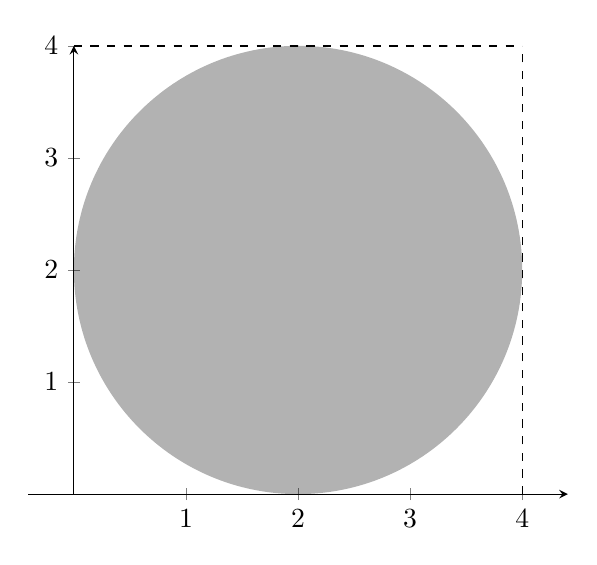
\begin{tikzpicture}
      \begin{axis}[
        xmin=0,
        xmax=4,
        ymin=0,
        ymax=4,
        axis equal,
        axis lines=middle,
        disabledatascaling]

      \fill [opacity=0.3] (2, 2) circle [radius=2];
      \addplot[thick, dashed, domain=0:4] {4};
      \addplot[dashed] coordinates{(4,0) (4,4)};
      \end{axis}
    \end{tikzpicture}
    \caption{A circle with center (2, 2) and radius 2 used in the sample calculation} \label{fig:circle}
  \end{figure}

  The circle is centered at (2, 2) and has radius 2. Thus the equation for the circle is given with
  \[ (x-2)^2 + (y-2)^2 = 4 \]
  The domain of possible inputs consists of the square bounded by the x and y axes and the lines
  $x = 4$ and $y = 4$ as represented by the dashed lines in Figure \ref{fig:circle}. \\

  Now a computer program can be written to generate several thousands points within the domain.

\end{document}
